\documentclass[journal,compsoc]{IEEEtran}
%DIF LATEXDIFF DIFFERENCE FILE
%DIF DEL main-oldtmp-1273.tex   Wed Oct 28 12:33:33 2015
%DIF ADD main.tex               Wed Oct 28 09:54:43 2015
\pagenumbering{arabic}

\usepackage{booktabs}
\usepackage{multirow}
%\usepackage{graphix}
\usepackage{lscape}

\usepackage{amssymb}
\usepackage{amsmath}
\usepackage{balance}  % to better equalize the last page
\usepackage{graphicx} % for EPS, load graphicx instead
\usepackage{times}    % comment if you want LaTeX's default font
\usepackage{url}      % llt: nicely formatted URLs
\usepackage[lofdepth,lotdepth]{subfig}
%\usepackage[pdftex]{hyperref}
\usepackage{multirow}
\usepackage{bbm}
\usepackage{pseudocode}
\usepackage{color}
%\usepackage{cite}
%\usepackage{algorithmic}
%\usepackage{algorithm}
%\usepackage[noend]{algpseudocode}
%\usepackage{algorithm}
\usepackage{algpseudocode}
\usepackage[linesnumbered,boxed,ruled]{algorithm2e}

%\newcommand{\modf3}[1]{\textcolor{blue}{#1}}

\newcommand{\TheName}{\mbox{\emph{Daehr}}}
\newcommand{\modif}[1]{\textcolor{blue}{#1}}
%DIF PREAMBLE EXTENSION ADDED BY LATEXDIFF
%DIF UNDERLINE PREAMBLE %DIF PREAMBLE
\RequirePackage[normalem]{ulem} %DIF PREAMBLE
\RequirePackage{color}\definecolor{RED}{rgb}{1,0,0}\definecolor{BLUE}{rgb}{0,0,1} %DIF PREAMBLE
\providecommand{\DIFadd}[1]{{\protect\color{blue}\uwave{#1}}} %DIF PREAMBLE
\providecommand{\DIFdel}[1]{{\protect\color{red}\sout{#1}}}                      %DIF PREAMBLE
%DIF SAFE PREAMBLE %DIF PREAMBLE
\providecommand{\DIFaddbegin}{} %DIF PREAMBLE
\providecommand{\DIFaddend}{} %DIF PREAMBLE
\providecommand{\DIFdelbegin}{} %DIF PREAMBLE
\providecommand{\DIFdelend}{} %DIF PREAMBLE
%DIF FLOATSAFE PREAMBLE %DIF PREAMBLE
\providecommand{\DIFaddFL}[1]{\DIFadd{#1}} %DIF PREAMBLE
\providecommand{\DIFdelFL}[1]{\DIFdel{#1}} %DIF PREAMBLE
\providecommand{\DIFaddbeginFL}{} %DIF PREAMBLE
\providecommand{\DIFaddendFL}{} %DIF PREAMBLE
\providecommand{\DIFdelbeginFL}{} %DIF PREAMBLE
\providecommand{\DIFdelendFL}{} %DIF PREAMBLE
%DIF END PREAMBLE EXTENSION ADDED BY LATEXDIFF

\begin{document}
\title{\TheName{}: a Linear Discriminant Analysis Framework for Electronic Health Record Data \\
 {\LARGE with its Application to Early Detection of Mental Health Disorders}}

\author{\IEEEauthorblockN{Haoyi Xiong,~Jinghe Zhang,~Yu Huang,~Kevin Leach, and ~Laura E. Barnes}~\thanks{Authors are all with Department of Systems and Information Engineering, University of Virginia, VA. Email:\{hx6d, xxx, xxx, xxx\}@virginian.edu}
}

\IEEEcompsoctitleabstractindextext{
\begin{abstract}
Electronic Health Records (EHR), consisting of massive patients'  diagnosis records, have been used to predict patients' future or potential diseases according to their past diagnoses. While tons of data mining tools have been adopted for EHR-based disease early detection, Linear Discriminant Analysis (LDA) is one of the most commonly used statistical methods. However, it is hard to train an accurate LDA model to early detect specific diseases when the known patients with the targeted diseases are few and the EHR data are coded manually with noise, since in such case the covariance matrices used in LDA are usually singular and estimated with large variance.
 %
With above issues in mind, this paper presents \TheName\ -- an extending LDA framework using Electronic Health Records. Beyond the existing LDA analyzers, \TheName\ is proposed to 1) eliminate the data noise caused by the manual encoding of EHR data, and 2) lower the variance of LDA model even when only a few patients' EHR are given for training. To achieve the two goals, we designed an iterative algorithm to improve the covariance matrix estimation with embedded data noise/variance reduction for LDA. We evaluated \TheName\ extensively using a large-scale real-world EHR dataset -- CHSN. Specifically, our experiments compared the performance of LDA to the three baselines (i.e., LDA and its derivatives),  in terms of identifying high risk college students potentially with mental health disorders from 23 US universities. Experiment results showed \TheName\ significantly outperformed three baselines by achieving 3\%--10\% higher prediction accuracy, and 3\% --14\% higher F1-score.

\end{abstract}

\begin{IEEEkeywords}
predictive models, early detection, anxiety/depression, temporal order, electronic health data
\end{IEEEkeywords}
}
\maketitle
\IEEEpeerreviewmaketitle

% For peer review papers, you can put extra information on the cover
% page as needed:
% \ifCLASSOPTIONpeerreview
% \begin{center} \bfseries EDICS Category: 3-BBND \end{center}
% \fi
%
% For peerreview papers, this IEEEtran command inserts a page break and
% creates the second title. It will be ignored for other modes.
\IEEEpeerreviewmaketitle

\section{Introduction}

With the rapid development of medical big data, forecasting future or potential disease based on patients' past medical records becomes a promising way to detect and further prevent high risk disease in advance.
Instead of paying attentions (e.g., screening or counseling)  to all its patient intensively, a medical system can predict each patient's potential diseases using his or her past diagnoses as well as the diagnoses records collected from massive other patients.
In this way, the medical system can identify high risk patients from the all patients with low cost, then serve patients in a targeted manner, further start prevention in advance.
Therefore, the accuracy of disease early detection is a crucial factor to improve the efficiency of high risk patient identification and disease prevention.Test


In this paper we present \TheName---an extending linear discriminant analysis (LDA)~\cite{fisher1936use,mclachlan2004discriminant} framework for disease early detection using Electronic Health Records (EHR), which can improve the prediction accuracy of the standard LDA model through reducing the noise in EHR data and regularizing the estimated covariance matrices.
In the rest of this section, we first discuss the motivations and background of this research, then we formulate a new research problem based on our observations and assumptions.
We elaborate the technical challenges of the proposed research and finally we summarize our technical contributions.


\subsection{Motivations and Backgrounds}

In order to predict patients' potential disease according to their past medical records, a variety of predictive models utilizing heterogeneous medical data have been studied~\cite{soni2011predictive,palaniappan2008intelligent,kumari2011comparative}, such as chest imaging for chest cancer early detection, questionnaire-based assessment (e.g., PHQ-9~\cite{kroenke2002phq}) data for mental disorder prediction, and screening data for heart disease prediction~\cite{d2001validation}.
Among all these medical data, Electronic Health Records (EHR) consisting of the diagnosis records of patients' each visit are used as a general purpose data source that enables massive disease early detection based on the previous diagnoses.
Furthermore, this data has a higher accessibility to clinicians and researchers and holds comprehensive information of patients medical history especially within the primary care setting.
Thus, EHR data also provides a promising opportunity for the disease early detection due to its general-purposeness, accessibility and standardized use and features. 


As shown in Fig~\ref{fig:exp-ehr}, a patient's EHR data includes all his/her past diagnosis and treatment records, where the diagnosis record includes a sequence of visits and each visits consists of multiple diagnoses.Please note that all diagnoses are recorded using ICD-9 codes~\cite{dubberke2006icd}, where each evidence of diagnosis corresponds to a specific ICD-9 code.
With diagnosis records in the EHR data, several methods~\cite{personalized2015, amarasingham2010automated, pittman2004integrated,jensen2012mining} have been studied to predict the disease of patients.
Given a disease as the prediction target (e.g., anxiety/depression) as well as the EHR data of a large population with/out the target disease, most of existing methods first represent each given patient's EHR data using a set of features, and then train a predictive model using features and labels (if each patient is diagnosed with the targeted disease) in a supervised manner.
Further, given each new patient's EHR data, these models predict if the given patient will develop the targeted disease in near future using the trained predictive model.


\begin{figure}
\centering
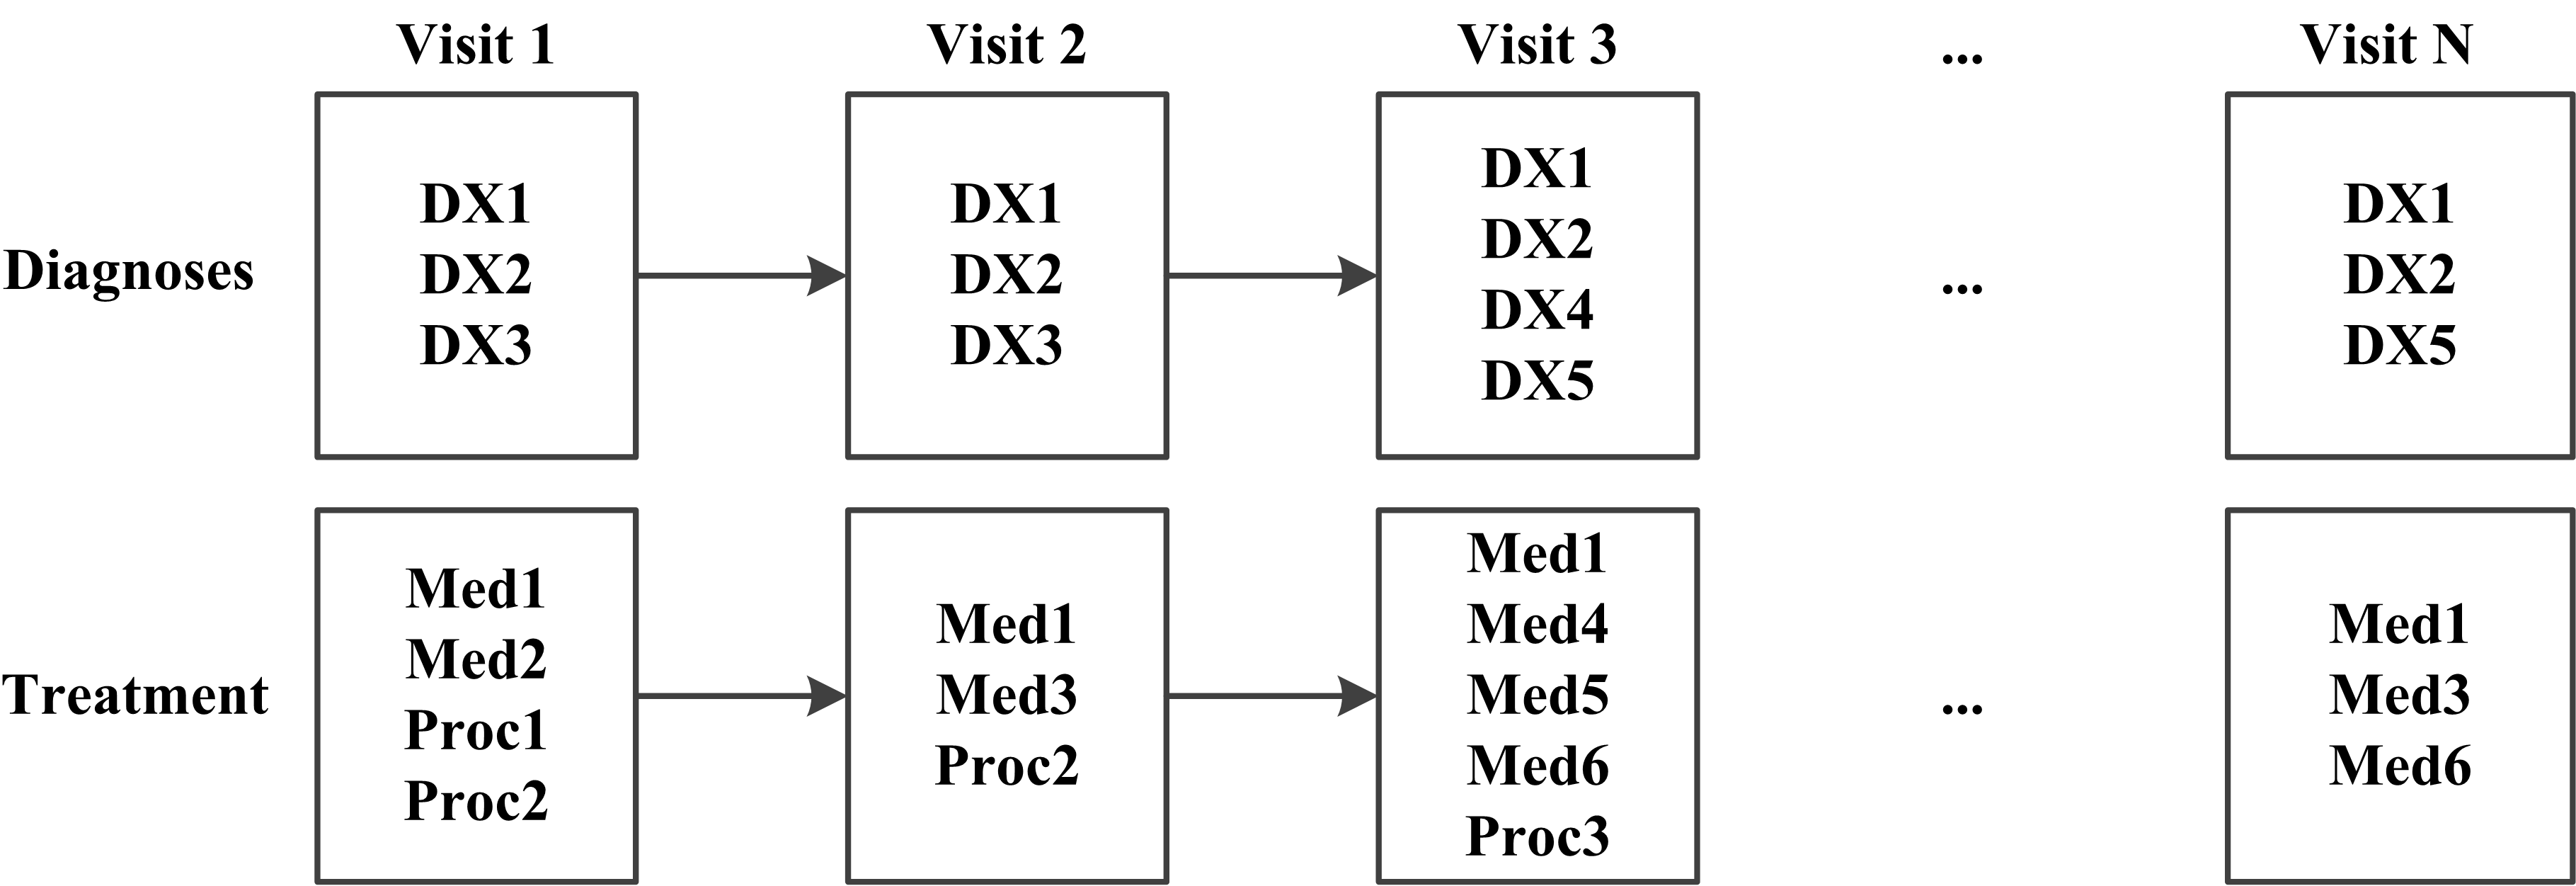
\includegraphics[width=0.48\textwidth]{./img/Patient.png}
\caption{An Example of a Patient's EHR Data}
\label{fig:exp-ehr}
\end{figure}


\textbf{EHR Data Representation for Early Detection.} 
In terms of representing EHR data, existing approaches include using diagnosis-frequencies~\cite{sun2012supervised,7091853,personalized2015}, pairwise diagnosis transitions~\cite{zhang_mseq_2015,jensen2001mining}, graph representations of diagnosis sequences~\cite{liu_temporal_2015}, and so on.
Among these approaches, the diagnosis-frequency is considered as one of common ways to represent EHR data.
Given each patient's EHR data, which consists of the patient's demographic information and a sequence of past visits, existing methods first retrieve the diagnosis codes recorded during each visit.
Then, the frequency of each diagnosis appearing in all past visits are counted, followed by further transformation on the frequency of each diagnosis into a vector of frequencies (e.g., $\langle 1, 0, \dots, 3\rangle$, where 0 means the $2^{nd}$ diagnoses does not exist in all past visits).
In this way, each patient having different number of visits and each visit consisting of multiple diagnoses is represented as a fixed-length data vector, which can be handled by common machine learning algorithms.


Please note that the diagnosis-frequency representation of EHR data is usually with ultra-high dimensions; for example, there exists more than 15,000 ICD-9 codes in EHR scheme, thus the diagnosis-frequency vector using raw ICD-9 codes is usually with thousands of dimensions.
In order to reduce the dimensinality, clinical professionals may suggest to use clustered code set, where each ICD-9 code can map to  one of the 295 clustered codes.
In this way, each raw diagnosis-frequency vector can be compressed to a vector of around 200 dimensions using clustered codes.


\textbf{Supervised Learning for Early Detection.} 
Given an EHR database and a target disease for early detection, existing method usually needs to first select patients both with and without the disease, then use their EHR data with appropriate representation to form a training set.
In order to train an accurate predictive model with the training set, a lot of machine learning methods such as Support Vector Machine (SVM), Random Forest (RF), Bayesian Network, Gaussian Process and Linear Discriminant Analysis (LDA) have been adopted~\cite{sun2012supervised,7091853,personalized2015,zhang_mseq_2015,jensen2001mining,liu_temporal_2015,cazzanti_local_2007}.
Among these machine learning methods, LDA is frequently used as one of the common performance benchmarks in a series of studies~\cite{cazzanti_local_2007,zhang_mseq_2015,kalina2013selecting,karlsson2014handling,wang2014clinical}, considering its capacity of dimension reduction.
For example, when using diagnosis-frequency vector as the representation of EHR data, a LDA model learns a linear combination of diagnoses (from the all diagnoses) that can optimally separate patients into the two groups (i.e., with/without the disease).
Then LDA predicts if new patients will develop to the targeted disease through separating their vectors into the two groups using the linear combination.


Please be advised that, just like many other statistical learning models, the accuracy of a LDA model can be improved, when more samples are given for training.
It is because the decision risk of a LDA model is inherited from the variance of its training samples, while \emph{increasing the sample size lower the sample variance}~\cite{hsu1947complete,qiao2008effective}.
In contrast, when the training samples are few, the model even cannot produce any valid prediction results.
Because LDA needs to use the \emph{inverse of the covariance matrices} to predict, while in such case the covariance matrices estimated in LDA are singular or namely \emph{non-inversiable} (i.e., the inverse of the covariance matrix doesn't exist)~\cite{huang2002solving,gao2006direct}.


With above backgrounds in mind, we are motivated to enhance the supervised learning methods on top of EHR data, so as to improve the prediction accuracy for disease early detection.
Specifically, we attempts at studying the LDA model using the diagnosis-frequency features, considering the relevance of such settings in clinical practices.


\subsection{Research Assumptions and Objectives}

Our research is based on following two  observations and two assumptions about EHR data and early detection settings:

\textbf{Observation 1. EHR Encoding Variation - } 
In terms of EHR data encoding, the diagnosis records are usually inputted manually by clinicians without a unified encoding scheme.
Our previous work~\cite{xxx} finds that, for one patient, the diagnosis records for one disease might be more frequent than the times that the disease has been diagnosed.
For example, \emph{three clinicians--Ann, Bob and Carl are working in the same clinics.
Given a patient has been diagnosed with upper respiratory infection (ICD-9 code: 465.9), Ann may only leave the record  of code 465.9 in the first visit when the disease is diagnosed.
However Bob may leave the record in the first visit as well as all his/her returning visits to receive screening/treatment for upper respiratory infection; while Carl may leave in the first visit and some of the returning visits that he feels necessary.}  

\textbf{\em Assumption I. Non-negative Noise in Diagnosis-Frequency Vector Data - } 
With the first observation in mind, it is reasonable to assume that each diagnosis is recorded at least one time in EHR and the number of records might be differing from encoding clinicians (i.e., \emph{frequency of record $\geq$ frequency of diagnosis} for each specific disease).
In this case, we further assume the encoding variation of EHR data may cause certain unknown \emph{non-negative data noise} on top of the diagnosis-frequency vectors.


\textbf{Observation 2. Limited Positive Training Samples - } 
We find that the total number of patients with a specific disease or namely \emph{positive samples} might be so few to train a predictive model for early detection of the disease.
For example, \emph{a historically black college wants to identify the risk students in terms of mental health disorder using all students' EHR installed in the college clinics.
The clinics first sorts all students to two groups (i.e., with/without mental disorder diagnosed), then from each group it selects a subset of students as training samples.
However, due to the low utilization rate of psyclinics by African American, the available training samples with at least one type of mental disorders (e.g., depression, anxiety, mood and personality disorders) are so few (e.g., 100$-$500 students) in their school.}  

\textbf{\em Assumption II.  Decision Risk of LDA Model for Early Detection of Diseases - } 
Considering the dimension $p$ of diagnosis-frequency vectors (e.g., $p\geq 200$ using clustered code set), we assume that the size of positive samples for LDA training is relatively small i.e., $0<n\lll 2^p$, where $n$ refers to the number of positive training samples.
Please note that when $0<n<p$, the trained LDA model can not produce any valid prediction results, since the estimated covariance matrix is singular/non-inversiable; when $p\leq n\lll 2^p$ the trained LDA model might be able to produce the prediction result but with large decision risk inherited from the variance of small training samples.


With above two assumptions in mind, our work attempts at reducing the affect of noise while lowering the decision risk of the LDA model for early detection of diseases.
Specifically we use \emph{mental health disorders} as the ''target disease'' in evaluation and experiment design, with respect to  {\em Assumption II}.


\subsection{Technical Issues and Contributions} 
In order to improve LDA with respect to the two assumptions, we need to address following three technical issues:

\begin{enumerate} \item \textbf{\em Eliminating the data noise in diagnosis-frequency vectors caused by encoding variation - }      
Given the frequency-diagnosis vectors for training, LDA first estimates sample diagnosis-to-diagnosis covariance matrices using an unbiased estimator like \emph{Intrinsic Estimator} or \emph{Maximized Likelihood Estimator (MLE)}, then builds the predictive models using estimated covariance matrices.
However, our later analysis shows that the non-negative data noise in the vectors might make the estimated covariance matrices more dense than the noise-free (ideal) one.
In this way, there might need a method to \emph{sparsify} the covariance matrices in order to reduce the affect of data noise to LDA.



\item \textbf{\em Lowering the decision risk of LDA while guaranteeing non-singularity and positive definiteness of the estimated covariance matrices - }      
In order to lower the decision risk of LDA, one possible solution is to use the $\ell^1$-penalized estimation of the covariance matrices~\cite{cai2012minimax,xue2012positive}.
However, any modifications (including $\ell^1$-penalty and sparse approximation) to a coavriance matrix might loss its positive definiteness---we cannot use such modified matrix in the statistics model.
In this way, there needs an algorithm to obtain the $\ell^1$-penalized estimation of the sparsifed covariance matrix while ensuring the estimation is non-singular and positive semi-definite.


\item \textbf{\em Incorporating the newly-estimated covariance matrices for EHR-based LDA - }      
Given the non-singular/positive-definite $\ell^1$-penalized sparse estimations of the  covariance matrices, we might need to use them to replace the covariance matrices originally used in LDA.
Thus there needs a generic framework to extend the original LDA through incorporating the aforementioned covariance matrix estimation algorithms.


\end{enumerate}

With aforementioned research challenges in mind, we made following technical contributions in this study:

\begin{itemize}

    \item In this work, we studied the problem to improve the existing Linear Discriminant Analysis (LDA) for disease early detection based on our two assumptions.
To the best of our knowledge, this paper is the first work for LDA-based disease early detection on top of EHR data, by addressing the encoding variation and low training sample size issues.


\item In order to tackle the technical challenges aforementioned, we proposed \TheName---an extending LDA framework.
It takes a novel approach to eliminate the affect of data noise and lower the decision risk of LDA model  through estimating sparse and non-singular diagnosis-to-diagnosis covariance matrices from diagnosis-frequency vectors.
Theoretical analysis shows that, with low computational complexity, the proposed algorithm can approximate the $\ell^1$-penalized near-sparsest estimation of the diagnosis-to-diagnosis covariance matrices with non-singularity and positive semi-definiteness guaranteed, even when a very limited number of diagnosis-frequency vectors are given for LDA training.


\item We evaluated \TheName\ using a real-world dataset CHSN,  which contains more than 300,000 students' EHR records collected from 23 US universities in past three years.
We designed a set of experiments based on CHSN for large-scale mental health disorder early detection.
The evaluation results show \TheName\ significantly outperformed three baselines (i.e., LDA and its derivatives) by achieving 3\%--10\% higher prediction accuracy, and 3\%--14\% higher F1-score.


\end{itemize}


The paper is structured as follows: Section~\ref{sec:2} discusses the previous studies that have been done in the data mining approaches to early detection of disease and LDA extensions.
Section~\ref{sec:3} introduces the problem formulation of our study and introduces the  \TheName\ framework to solved the problem.
Section~\ref{sec:4} describes two core algorithms used in \TheName.
Section~\ref{sec:5} describes the data used in this research, the experimental design, and the experimental results and analyses.
Finally, the summary of this work, future work, and clinical context are discussed in Section~\ref{sec:6}.



\section{Related Work}\label{sec:2}

% machine learning in medical area
In this section, we summarize the previous studies related to this paper from following two aspects: \emph{data mining approaches to early detection of diseases} and \emph{extensions to LDA learner}.

\subsection{Big Data Approaches to Disease Early Detection}
Various analytical methods have been used to study the causes, prevention, progression, and interventions of diseases, among which machine learning has become very promising in the prediction of diseases ~\cite{maroco_data_2011, huang_toward_2014}. In this section, we will discuss the related works in terms of the \emph{predictive modeling} and \emph{data representation} approaches.

\textbf{Predictive Models for Early Detection of Disease} Predictive models have become popular in the early detection of diseases, such as breast cancer, type II diabetes, cardiovascular disease, etc.~\cite{Lindstrom01032003, riskprediction, zheng_predictive_2015, yoo_data_2011} The outcome of the predictive models are beneficial to both care providers and patients. Accurate prediction of diseases can assist clinicians in identifying high-risk patients in an early stage ultimately leading to more timely diagnosis and focusing the resources to deliver effective treatment to those patients. In essence, the early detection of diseases can be viewed as a classification problem so that well-established classifiers can be used to perform the task. Among the studies on the early detection of mental disorders, a LASSO logistic regression model has been applied to predict the depression severity to help personalize treatment for high-risk patients~\cite{huang_toward_2014}. In this work, the feature vector used for prediction includes gender, ICD-9 codes, disease and drug ingredient terms, and average number of visits. However, the predictive model is more accurate in recognizing low risk-patients and achieves a 90\% specificity, while the sensitivity are 25\% using the information 12 months before the diagnosis and 50\% at the time of diagnosis, respectively~\cite{huang_toward_2014}.

\textbf{EHR Data Representation for Predictive Models. } Electronic health data is highly accessible in health care institutions and has become a promising data source for public health research. However, EHR data is heterogeneous and cannot be readily expressed in a unified vector space. Thus, an appropriate representation of those data is critical for further advancements in analytics and modeling. Many data representation approaches has been developed to preserve useful information from the raw data. Usually, frequency is used as the representations for categorical features of an instance, where presence or absence is used for binary variables~\cite{ng_personalized_2015, huang_toward_2014}. However, this representation omits the temporal orders of clinical events and an attempt has been made to incorporate the information by introducing pairwise transitions of diagnoses in addition to the widely used frequency features~\cite{zhang_mseq_2015}. In addition, some novel frameworks are proposed to learn the temporal knowledge in patients' sequences~\cite{wang_towards_2012, wang_framework_2012, liu_temporal_2015}. In~\cite{wang_framework_2012}, it uses a spatial-temporal matrix to represent the a sequence of events in which the two dimensions represents the event type and time information, respectively. In~\cite{liu_temporal_2015}, the events in a patient's EHR is represented by a temporal graph and basis graphs are learned as the features to represent patients. Furthermore, frequent sequence mining has been utilized to uncover the most important event sequences~\cite{gotz_methodology_2014, perer_frequence:_2014, perer_mining_2015}. In~\cite{gotz_methodology_2014}, it combines the episode definition and temporal pattern mining techniques to support the visual exploration of the most impactful clinical event patterns to outcome. To address high dimensional data, FeaFiner is proposed for simultaneous feature grouping and selection. Thus, it extracts relevant and non-overlapping feature concepts in a low dimensional space, where the prediction accuracy is improved when applied to predicting Alzheimer's Disease-related scores~\cite{zhou_feafiner:_2013}. 

\subsection{Extensions to LDA Model}
Regarding the application of LDA to EHR-based early detection of diseases, here we mainly introduce several LDA extensions under High Dimension Low Sample Size (HDLSS) settings. As aforementioned, when LDA works in HDLSS, there might exist two major technical issues: 1) LDA needs the inverse of covariance matrices for classification while covariance matrices estimated from small samples are usually singular (non-inversiable), and 2) large decision risk is inherited from the variance of small samples, through classical LDA training. In order to handle the singular (non-inversiable) covariance matrix issues,~\cite{ye2004optimization} proposed to use the Pseudo-inverse of the singular covariance matrix, while Direct LDA~\cite{lu2003face,gao2006direct} proposed to use the \emph{simultaneous diagonalization} of covariance matrices, which are non-singular, to replace the original covariance matrices. On the other hand,  ~\cite{clemmensen2011sparse,qiao2008effective,shao2011sparse} have been proposed to order to lower the decision risk through regularizing the estimated covariance matrices..

\TheName\ is different from above related work in the following aspects. First, compared to other data mining approaches to early detection of disease such as~\cite{Lindstrom01032003, riskprediction, zheng_predictive_2015, yoo_data_2011}, \TheName\ is the first work that intends to improve the performance of LDA model by addressing data noise and small positive training sample size issues. Second our contribution is complementary with those work in EHR data representation~\cite{wang_towards_2012, wang_framework_2012, liu_temporal_2015} and we are open to further improve \TheName\ by incorporating advanced EHR data representation methods.
%
Third, when compared to the existing LDA extensions, \TheName\ re-estimates the covariance matrices to (1)  eliminate the affect of data noise to LDA model, (2) lower the decision risk inherited from  small positive training samples, and (3) guarantee the non-singularity, while~\cite{ye2004optimization,lu2003face,gao2006direct,clemmensen2011sparse,qiao2008effective,shao2011sparse} focuses on regularizing the covariance matrices to enable LDA in a general HDLSS setting.  Thus the estimation/optimization problems considered in any single one of the previous studies are mathematically different from ours with different objectives and assumptions.

\section{\TheName{} System Model}\label{sec:3}
In this section, we first formulate the research problem of our study; then we propose \TheName\ framework to solve the formulated problem.

\subsection{Problem Formulations}
According to our research assumptions, in this section, we make two definitions and introduce several preliminary studies used in our studies. Further, we formulate our research problem based on all above definitions and preliminaries.

\textbf{\em Definition I.} \emph{Diagnosis-frequency Vector and Non-negative Noise Vector - } Given EHR data of $m$ patients (both with and without the targeted disease), we can extract $m$ diagnosis-frequency vectors $X_0,X_1\dots X_{m-1}$. Each vector e.g., $X_i=<1,0,\dots,3>$ consists of two parts: $\hat{X}_1$ the vector of true diagnosis frequencies (not diagnosis record frequencies) and $E_i$ the non-negative noise vector:
\begin{equation}
X_i=\hat{X}_1+E_i
\end{equation}

\textbf{\em Preliminary I. }\emph{Generalized Two-class LDA and Covariance Matrices - } According to the common implementation of a LDA classifier~\cite{ziegel2003modern}, given $m$  training samples as well as the labels i.e., $(X_0,l_0)\dots (X_{m-1},l_{m-1})$ where $l_i\in\{-1,+1\}$ refers to whether the patient $i$ has been diagnosed with the target disease (i.e., positive sample or negative sample),  a two-class LDA  model first sorts each sample into two groups according to the label, and estimates covariance matrix/mean vector of the two classes, i.e., ($\Sigma_{+}$, $\mu_+$) and ($\Sigma_{-}$,$\mu_-$), using the positive samples and negative samples respectively.  Then generalized two-class LDA determine if a new patient ($X'$) would develop to the targeted disease, using
%
\begin{equation}
\begin{aligned}
&(X'-\mu_-)^T\Sigma_{-}^{-1}(X'-\mu_-)+ln|\Sigma_-|-\\
&(X'-\mu_+)^T\Sigma_{+}^{-1}(X'-\mu_+)-ln|\Sigma_+|<T,
\end{aligned}
\label{eq:glda}
\end{equation}
%
where $T$ is an optimal threshold based on the training samples. However, as illustrated in our observation 2,  when positive sample size is relatively small e.g., for the rare disease in the database,  $Rank(\Sigma_+)<p$,  $\Sigma_{+}$ is singular and $\Sigma_{+}^{-1}$  doesn't exist. In this case, Equation~\ref{eq:glda} might not work.

Please note that in the rest of paper we name the both $\Sigma_{+}$ and $\Sigma_{-}$  as a \emph{covariance matrix} simply, since they are considered equally in our problem formulation and solution design; in contrast, the covariance matrix may refer to the either $\Sigma_{+}$ or $\Sigma_{-}$.

\textbf{\em Definition II.} \emph{Sample Diagnosis-to-Diagnosis Covariance Matrix Estimation and Disturbance of Non-negative Noise - } With above settings in mind, we further define $\Sigma$ as the sample diagnosis-to-diagnosis covariance matrix based on noisy data, $\hat{\Sigma}$ as the sample covariance matrix based on ``noisy-free'' vectors, and  $\Delta=\Sigma-\hat{\Sigma}$ as the disturbance of non-negative noise to covariance estimation.
%
\begin{equation}
\begin{aligned}
\Sigma&=\frac{1}{n}\sum_{i=0}^{n-1} X_iX_i^T
=\frac{1}{n}\sum_{i=0}^{n-1} (\hat{X}_i+E_i)(\hat{X}_i+E_i)^T\\
&=\hat{\Sigma}+\Delta
\end{aligned}
\label{eq:sample-cov}
\end{equation}
As the sample covariance matrix estimation shown in~\ref{eq:sample-cov}, the disturbance should be:
%
$$\Delta=\frac{1}{n}\sum_{i=0}^{n-1}(2\hat{X}_iE_i^T+E_iE_i^T).$$ 
%
According to our definition $\hat{X}_i$ and $E_i$ are both non-negative matrices, it is not hard to find that $\Delta=\Sigma-\hat{\Sigma}\geq \textbf{0}$ is a non-negative matrix and $||\Sigma||\geq ||\hat{\Sigma}||$. Thus, we can roughly conclude that $\hat{\Sigma}$ might be a sparse estimation of $\Sigma$. 

\textbf{\em Preliminary II. } \emph{Minimax decision risk estimation of the covariance matrix in HDLSS settings.} Previous work~\cite{cai2012minimax,xue2012positive} showed that it is possible to achieve \emph{minimax risk} covariance matrix estimation from a few samples, using the \emph{minimal $\ell^1$-normal estimation} of the original sample covariance matrix. In this case, in terms of lowering variance of LDA, we can assume that the optimal~\cite{cai2012minimax} covariance matrix $\tilde{\Sigma}$ should be a $\ell^1$-penalized sparse estimation of $\hat{\Sigma}$.

\textbf{Problem Formulation. } According to above definitions and preliminaries, this paper considers a problem of finding the positive-definite sparse estimation of $\hat{\Sigma}$--the noisy-free diagnosis-to-diagnosis covariance matrices, to improve the performance of LDA for early detection of disease. Hereby, we define our research problem that, Given $n$ diagnosis-frequency vectors $X_0,X_1\dots X_{n-1}$,  our problem is to estimate $\tilde{\Sigma}$:
\begin{equation}
\begin{aligned}
\text{min. }|\tilde{\Sigma}|_1 \text{ s.t. }||\tilde{\Sigma}-\hat{\Sigma}||_F^2\leq \epsilon\text{ and }\tilde{\Sigma}\in {\bf }I^+
\end{aligned}
\label{eq:problem}
\end{equation}
where ${\bf }I^+$ refers to the overall set of positive semi-definite matrices. Please note that $\hat{\Sigma}$ is not foreknown due to the unknown data noise. 

Intuitively, it is possible to solve the formulated problem through sparsifying and regularizing the sample diagnosis-to-diagnosis covariance matrix $\Sigma$ subject to the positive semi-definite and non-singularity constraint. 


\begin{figure}
\begin{center}
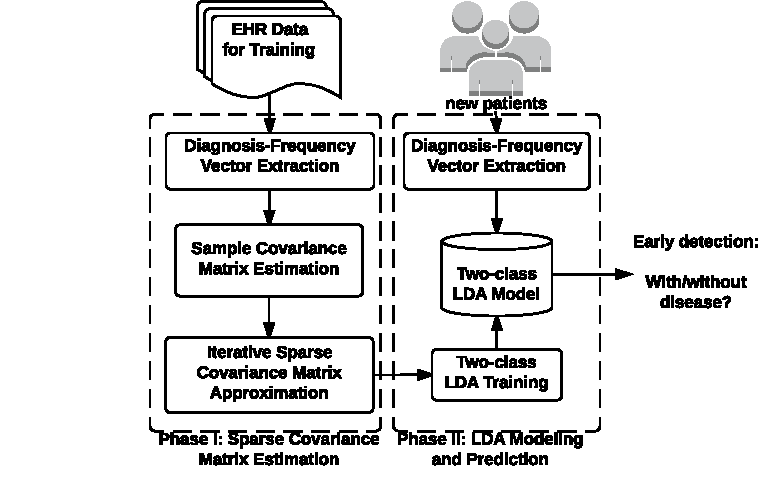
\includegraphics[width=0.48\textwidth]{./img/daehr.pdf}
\end{center}
\caption{\TheName\ Framework}
\end{figure}


\subsection{\TheName\ Framework}
In this section, we introduce the framework design of \TheName. The framework of \TheName\ consists of two phases, which first uses the EHR data for training to estimate the covariance matrices used in LDA w.r.t our problem formulation, then adopts LDA  with newly-estimated parameters to predict if the new patient will develop the targeted disease.

\emph{Phase I: Sparse Covariance Matrix Estimation - } Given the patients' EHR data as training set, this phase estimates the sparse covariance matrices for two classes of patients with following two steps:
\begin{enumerate}
\item \textbf{Diagnosis-frequency Vector Extraction and Sample Covariance Matrix Estimation - } \TheName\ first convert each patient's EHR data to a diagnosis-frequency vector and combine it with his/her label (indicating if the patient has been diagnosed with/without the targeted disease) i.e.,  $(X_0,l_0)\dots (X_{m-1},l_{m-1})$ where $l_i\in\{-1,+1\}$ as the label of the $i^{th}$ patient. With the vectors of two classes, \TheName\ then estimates the sample covariance matrices for the two classes $\Sigma_+$ and $\Sigma_-$ using Eq.~\ref{eq:sample-cov}.

\item \textbf{Iterative Sparse Covariance Matrix Approximation - } Given sample covariance matrices $\Sigma_+$ and $\Sigma_-$, \TheName\ estimates the positive-definite $\ell^1$-penalized estimation of both $\Sigma_+$ and $\Sigma_-$ using a unified iterative approximation process, where \TheName\ treats $\Sigma_+$ and $\Sigma_-$ equally. As shown in Alg.~\ref{alg:iap}, given an input sample covariance matrix $\Sigma_0=\Sigma_+$ or $\Sigma_-$, the process iteratively approximates to the positive definite $\ell^1$-penalized estimation of $\Sigma_0$, through alternating two algorithms -- \emph{$\ell^1$-penalized Sparse Matrix Estimation} and \emph{Nearest Positive Semi-Definite Matrix Approximation} in each iteration. In Alg~\ref{alg:iap}, $\Delta'=\frac{||\Sigma_{t+1}-\Sigma_{t}||_\infty}{||\Sigma_{t}||_\infty}$ and $tol$ is a threshold characterizing the tolerance of convergence. Specifically, in each (e.g., the $t^{th}$, $t\geq 0$) iteration  iteration, the process obtains an improved result $\Sigma_{t+1}$ using the previous result $\Sigma_{t}$. With the result improved iteration by iteration, the algorithm stops only when the predefined convergence achieved $\Delta''< tol$ or maximal iterations reached $t>maxit'$.

\end{enumerate}
Please note that the covariance matrices for the two classes of patients are estimated in this phase through an unified process, we denote the new covariance matrices as $\Sigma_+^*$ and $\Sigma_-^*$ for the positive and negative classes respectively.

\begin{algorithm}
\caption{Iterative Approximation Process for Sparse Covariance Matrix Estimation}
\label{alg:iap}
\KwData{$\Sigma_{0}$ -- the sample covariance matrix i.e., $\Sigma_+$ or $\Sigma_-$}
\KwResult{${\Sigma_{t+1}}$ -- the positive definite $\ell^1$-penalized estimation of $\Sigma_0$}
\Begin{
\While{ $\Delta' \geq tol, \text{ or }0\leq t \leq maxit'$  }{
	$\Sigma_{t+\frac{1}{2}}\gets \ell^1$-penalized sparse estimation of $\Sigma_t$
    $\Sigma_{t+1}\gets $ the nearest positive semi-definite approximation to  $\Sigma_{t+\frac{1}{2}}$
}
\Return{$\Sigma_{t+1}$}
}
\end{algorithm}


\emph{Phase II: LDA Modelling and Prediction - } Given the two estimated matrices $\Sigma_+$ and $\Sigma_-$ as well as the training samples, this phase first trains the optimal model for LDA prediction and then uses the LDA model for new patients prediction. This phase consists of following two steps:
\begin{enumerate}
\item \textbf{LDA Model Training - } Given the two estimated covariance matrices $\Sigma_+^*$ and $\Sigma_-^*$ as well as training samples $(X_0,l_0)\dots (X_{m-1},l_{m-1})$, \TheName\ searches the optimal threshold $T^*$ that can maximally classify the two classes of samples with Eq.~\ref{eq:glda}. In this case, \TheName\ models a LDA model as $(\Sigma_+^*,\mu_+,\Sigma_-^*,\mu_-,T^*)$.
\item \textbf{LDA-based new Patient Prediction - } Given a new patient's EHR data, \TheName\ first convert her data to diagnosis-frequency vector e.g., $X'$. Then together with the LDA model described as $(\Sigma_+^*,\mu_+,\Sigma_-^*,\mu_-,T^*)$, \TheName\ predict if the patient will develop the targeted disease using the criterion in Eq.~\ref{eq:glda}.
\end{enumerate}
%

After above two phases terminate, \TheName\ has learned a LDA model with advanced covariance matrices estimation, then adopted the LDA model to enable the early detection of targeted disease. Though the whole framework has beens sketched, the design of some algorithms have not yet been introduced. The design of aforementioned \emph{$\ell^1$-penalized Sparse Matrix Estimation} and \emph{Nearest Positive Semi-Definite Matrix Approximation} algorithms are discussed in following sections.

\section{\TheName\ Core Algorithms}~\label{sec:4}
In this section, we first introduce the two core algorithm used in \TheName, then analyzes the performance of the proposed algorithms.

\subsection{$\ell^1$-penalized Sparse Matrix Estimation}
Given the covariance matrix estimated in the previous iteration $\Sigma_{t}$, this algorithm estimates $\Sigma_{t+\frac{1}{2}}$ -- the $\ell^1$-penalized sparse estimation of $\Sigma_{t}$, using the Proximal Gradient Descent algorithm~\cite{nesterov2004introductory} with following objective function:   
\begin{equation}
\emph{min. }\frac{1}{2}||\Sigma_{t+\frac{1}{2}}-\Sigma_t||_F^2+\tau |\Sigma_{t+\frac{1}{2}}|_1,
\label{eq:sparse-imp}
\end{equation}
where $\tau$ is a Lagrange multiplier~\cite{wu2009karush}. When $\tau\geq 0$, the Eq.~\ref{eq:sparse-imp} is a \emph{convex function with sparse input} which can be optimally converged using proximal gradient descent~\cite{nesterov2004introductory}. Please note that $\Sigma_{t+\frac{1}{2}}$ is neither symmetric nor positive semi-definite.



\subsection{Nearest Positive Semi-Definite Matrix Approximation}
Given the sparse matrix $\Sigma_{t+\frac{1}{2}}$, we intend to approximate its nearest positive-definite matrix $\Sigma_{t}$ (the output of the $t^{th}$ iteration) as Equation~\ref{eq:nearest-pd}. 
%
\begin{equation}
\emph{min. } ||\Sigma_{t+1}-\Sigma_{t+\frac{1}{2}}||_F^2 \emph{ s.t. }\Sigma_{t+1}\in  {\bf }I^+
\label{eq:nearest-pd}
\end{equation}
%
In order to achieve the goal, we use the Alternating Projection Algorithm~\cite{higham2002computing} shown in Alg~\ref{alg:apm}. Specifically, the projection $P_S(A)=\frac{1}{2}(V\lambda_+V^T+(V\lambda_+V^T)^T)$ and  $\lambda_+=\langle min\{\lambda_0,0\},min\{\lambda_1,0\}\dots  \rangle$, where $V,\lambda_i$ is the eigenvalue decomposition of $A$; the projection $P_U(A)=A'$, where $A'_{i,j}=1$ when $i=j,$ and $A'_{i,j}=A_{i,j}$ when $i\neq j$; the stopping criterion $\Delta''=max\{\frac{||H_{k+1}-H_k||_\infty}{||H_k||_\infty}, \frac{||H_{k+1}^*-H_k^*||_\infty}{||H_k^*||_\infty}, \frac{||H_{k+1}^*-H_k^*||_\infty}{||H_k||_\infty}\}$.


The algorithm stops when the predefined convergence achieved $\Delta'' < tol$, or maximal iterations reached $k= maxit''$. Please note that when the algorithm stops at any $k> 0$, the output $\Sigma_{t+1}$ must be a positive semi-definite matrix; while when $k\to+\infty$, the output $\Sigma_{t+1}$ could converge to the optimal solution~\cite{dykstra1983algorithm} of the optimization problem addressed in Eq.~\ref{eq:nearest-pd}.

\begin{algorithm}
\caption{Alternating Projection Algorithm for Nearest Positive Definite Matrix Approximation}
\label{alg:apm}
\KwData{$\Sigma_{t+\frac{1}{2}}$ -- the $\ell^1$-penalized sparse estimation of $\Sigma_{t}$, $tol$ -- the tolerance of convergence}
\KwResult{$\Sigma_{t+1}$ -- the nearest positive definite approximation to $\Sigma_{t+\frac{1}{2}}$}
\Begin{
 {\bf initialization:}\\
  $H_0$ = $\frac{1}{2}(\Sigma_{t+\frac{1}{2}}+\Sigma_{t+\frac{1}{2}}^T)$, $k = 1$, $I_{mod_0} = 0$, $\Delta = 1$;\\
\While{ $\Delta'' \geq tol, \text{ or } 0\leq k \leq maxit''$  }{
 $R_{k+1} = H_{k} - I_{mod_{k}}$, \\%\% $I_{mod_{k-1}}$ is Dykstra's correction;\\
 $H_{k+1}^{*} = P_S(R_{k+1})$;\\
 $I_{mod_{k+1}} = H_{k+1}^{*} - R_{k+1}$;\\
 $H_{k+1} = P_U(H_{k+1}^{*})$;
}
$\Sigma_{t+1}=H_{k+1}$\\
\Return{$\Sigma_{t+1}$}
}
\end{algorithm}


\subsection{Algorithm Analysis}
\section{Evaluation}\label{sec:5}
% why study mental health disorders?
In this  section, we first introduce the experiment design of our evaluation, then we introduce the experiment results, including the performance comparison between \TheName\ and original LDA baselines, as well as the performance comparison between \TheName\ and other predictive models. Finally, we compare the time consumption of \TheName\ to other models.



\subsection{Experiment Design}
We first present the datasets used for \TheName\ evaluation, then introduce the targeted diseases for the early detection, further we specify the settings of early detection.

\textbf{Dataset for Evaluation - } In this study, to evaluate \TheName, we plan use the de-identified EHR data from the College Health Surveillance Network (CHSN) which contains over 1 million patients and 6 million visits from 31 student health centers across the US~\cite{turner_college_2015}. In the experiments, we use the EHR data from 10 participating schools. The available information includes ICD-9 diagnostic codes, CPT procedural codes and limited demographic information. There are over 200,000 enrolled students in those 10 schools representing all geographic regions of the US. The demography of enrolled students (sex, race/ethnicity, age, undergraduate/graduate status) closely matched the demography for the population of US universities.

\textbf{Targeted Disease for Early Detection - } Among all diseases recorded in CHSN, we choose mental health disorders, including \emph{anxiety disorders, mood disorders, depression disorders and other related disorders}, as the targeted disease for early detection. Specifically, we plan to evaluate \TheName\ using the early detection of mental health disorders in \emph{college students}, considering following issues:
\begin{enumerate}
\item  \emph{Emergency of early detection of mental health disorders - } Mental health disorders have become a severe problem in the United States and many other countries that 18.6\% adults are with at least one mental disorders. According to the Spring 2014 American College Health Association's National College Health Assessment report, approximately half of the college students have had the feeling of hopeless and overwhelming anxiety~\cite{ACHA2014}. 

\item  \emph{Difficulty to recognize mental health disorders in early stage - } Mental health disorders are unrecognized frequently in primary care that untimely treatment results in emotional, physical, economic, and social burdens to patients and others. 

\item \emph{Limitation of common approaches to early detection of mental health disorders - } Questionnaires are commonly used to detect mental health disorders. Usually, specific questionnaires, interviews, or standard measurement are designed by researchers to collect patients' behavioral information targeting on a particular psychiatric disorder. In particular, psychological screening, PHQ-9, is used to evaluate a patient's risk of mental health disorders~\cite{kroenke2002phq}. However, these approaches are not generally applicable in primary care thus cannot detect mental disorders at an early stage. 

\end{enumerate}
%
With all above in mind, we are motivated to use EHR data for the early detection of mental health disorders, considering the accessibility and information contained in EHR. 

\textbf{Early Detection Settings - } From the CHSN datasets, we select 21,097 patients with anxiety/depression in the target group and 327,198 patients without any mental health disorder in the control group. We represent each patient using his/her diagnosis-frequency vector based on the clustered codeset, where four clustered codes (i.e., xxx, xxx, xxx, xxx) are considered to represent the diagnoses of mental health disorders. Specifically, if a patient has any of these four codes in his/her EHR, we consider he/she has been diagnosed with mental health disorders as ground truth. Please note that in our research, we don't intend to predict these four types of mental disorders separately, as these four disorders are usually correlated and heavily overlapped in clinical practices.


\begin{table*}
{
\begin{center}
\caption{Performance Comparison between \TheName\ and LDA Baselines (Testing Sample Size =$200\times 2$)}
		\label{tab:table11}
\begin{tabular}{*{10}{c}}
\toprule
    & & \multicolumn{8}{c}{Training Set $\times 2$}\\
    \cmidrule(lr){3-10}
    & & 
    \multicolumn{2}{c}{50} &
  %  \multicolumn{3}{c}{100} &
    \multicolumn{2}{c}{150} &
  % \multicolumn{3}{c}{200} &
    \multicolumn{2}{c}{250} &
  % \multicolumn{3}{c}{300} &
    \multicolumn{2}{c}{350} \\
\cmidrule(lr){3-4}
\cmidrule(lr){5-6}
\cmidrule(lr){7-8}
\cmidrule(lr){9-10}
Algorithm & Parameters & \texttt{Accuracy} & \texttt{F1-Score} & 
									   	 \texttt{Accuracy} & \texttt{F1-Score} & 
                          			 \texttt{Accuracy} & \texttt{F1-Score} & 
                           			 \texttt{Accuracy} & \texttt{F1-Score} \\
 \cmidrule(lr){1-2}                        
\cmidrule(lr){3-4}
\cmidrule(lr){5-6}
\cmidrule(lr){7-8}
\cmidrule(lr){9-10}
    LDA & N/A &   0.547 & 0.539   &     0.617 & 0.612       & 0.639 & 0.644      & 0.661 & 0.670 \\

\cmidrule(lr){1-2}                        
\cmidrule(lr){3-4}
\cmidrule(lr){5-6}
\cmidrule(lr){7-8}
\cmidrule(lr){9-10}
    DIAG & N/A &   0.592 & 0.591 &      0.635 & 0.635 &      0.639 & 0.639&   0.653 & 0.660    \\
   % \midrule
    \cmidrule(lr){1-2}                        
\cmidrule(lr){3-4}
\cmidrule(lr){5-6}
\cmidrule(lr){7-8}
\cmidrule(lr){9-10}

    \multirow{3}{*}{Shrinkage($\beta$)} 
& 0.25 &   0.593& 0.592 &      0.636 & 0.638      & 0.640 & 0.643      & 0.656 & 0.665      \\
& 0.50 &   0.594 & 0.592 &      0.630 & 0.630    & 0.641 & 0.645     & 0.660 & 0.669     \\
& 0.75 &   0.592 & 0.590 &      0.626 & 0.624    & 0.639 & 0.643      & 0.662 & 0.672   \\
    % \midrule
\cmidrule(lr){1-2}                        
\cmidrule(lr){3-4}
\cmidrule(lr){5-6}
\cmidrule(lr){7-8}
\cmidrule(lr){9-10}
     \multirow{5}{*}{\TheName($\tau$)} 
     & $0.005*0.5^{0}$ &   0.644 & 0.692 &     \textbf{0.667} & 0.714      & \textbf{0.662} & \textbf{0.716}     & \textbf{0.670} & \textbf{0.722}    \\
     & $0.005*0.5^{1}$ &   0.645 & 0.694 &     0.666 & 0.713      & \textbf{0.662} & \textbf{0.716}    & \textbf{0.670} & \textbf{0.722}    \\     
     & $0.005*0.5^{2}$ &   \textbf{0.646} & \textbf{0.697} &  0.663 & 0.714      & \textbf{0.662} & \textbf{0.716}     & \textbf{0.670} & \textbf{0.722}  \\
     & $0.005*0.5^{3}$ &   \textbf{0.646} & 0.694 &     0.661 & 0.712     & \textbf{0.662} & \textbf{0.716}     & \textbf{0.670} & \textbf{0.722}   \\
     & $0.005*0.5^{4}$ &   \textbf{0.646} & 0.696 &     0.662 & \textbf{0.715}     & \textbf{0.662} & \textbf{0.716}     & \textbf{0.670} & \textbf{0.722}  \\

     \bottomrule

\end{tabular}

\end{center}
}
\end{table*}


\begin{table*}
{
\begin{center}
\caption{Performance Comparison between \TheName\ and LDA Baselines  (Testing Sample Size =$1000\times 2$)}
		\label{tab:table12}
\begin{tabular}{*{10}{c}}
\toprule
    & & \multicolumn{8}{c}{Training Set $\times 2$}\\
    \cmidrule(lr){3-10}
    & & 
    \multicolumn{2}{c}{50} &
  %  \multicolumn{3}{c}{100} &
    \multicolumn{2}{c}{150} &
  % \multicolumn{3}{c}{200} &
    \multicolumn{2}{c}{250} &
  % \multicolumn{3}{c}{300} &
    \multicolumn{2}{c}{350} \\
\cmidrule(lr){3-4}
\cmidrule(lr){5-6}
\cmidrule(lr){7-8}
\cmidrule(lr){9-10}
Algorithm & Parameters & \texttt{Accuracy} & \texttt{F1-Score} &
						\texttt{Accuracy} & \texttt{F1-Score} &
                           \texttt{Accuracy} & \texttt{F1-Score}  &
                           \texttt{Accuracy} & \texttt{F1-Score}  \\
 \cmidrule(lr){1-2}                        
\cmidrule(lr){3-4}
\cmidrule(lr){5-6}
\cmidrule(lr){7-8}
\cmidrule(lr){9-10}
    LDA & N/A &   0.552 & 0.545  &     0.619 & 0.620      & 0.644 & 0.648      & 0.656 & 0.663  \\

     \cmidrule(lr){1-2}                        
\cmidrule(lr){3-4}
\cmidrule(lr){5-6}
\cmidrule(lr){7-8}
\cmidrule(lr){9-10}
    DIAG & N/A &   0.595 & 0.588  &     0.624 & 0.625      & 0.641 & 0.642     & 0.653 & 0.662  \\
   % \midrule
    \cmidrule(lr){1-2}                        
\cmidrule(lr){3-4}
\cmidrule(lr){5-6}
\cmidrule(lr){7-8}
\cmidrule(lr){9-10}

    \multirow{3}{*}{Shrinkage($\beta$)} 

& 0.25 &   0.596 & 0.592  &     0.629 & 0.631     & 0.644 & 0.648      & 0.657 & 0.667     \\   			& 0.50 &   0.594 & 0.589 &     0.630 & 0.633      & 0.646 & 0.649     & 0.660 & 0.670     \\
& 0.75 &   0.590 & 0.584  &     0.629 & 0.632     & 0.647 & 0.650     & 0.660 & 0.668     \\
    % \midrule
     \cmidrule(lr){1-2}                        
\cmidrule(lr){3-4}
\cmidrule(lr){5-6}
\cmidrule(lr){7-8}
\cmidrule(lr){9-10}
     \multirow{5}{*}{\TheName($\tau$)} 
     & $0.005*0.5^{0}$ &   0.653 & 0.711 &     \textbf{0.655} & \textbf{0.716}      & 0.666 & 0.718     & \textbf{0.667} & \textbf{0.720}    \\
     & $0.005*0.5^{1}$ &   0.653 & 0.711  &     \textbf{0.655} & \textbf{0.716}      & 0.666 & 0.718      & \textbf{0.667} & \textbf{0.720}   \\     
     & $0.005*0.5^{2}$ &   \textbf{0.653} & \textbf{0.712} &     \textbf{0.655} & \textbf{0.716}      & 0.666 & \textbf{0.720}     & \textbf{0.667} & \textbf{0.720}  \\
     & $0.005*0.5^{3}$ &   0.652 & 0.710  &     \textbf{0.655} & \textbf{0.716}      & 0.666 & 0.719     &\textbf{0.667} & \textbf{0.720}    \\
     & $0.005*0.5^{4}$ &   0.652 & 0.710  &     \textbf{0.655} & \textbf{0.716}       & \textbf{0.667} & \textbf{0.720}     & \textbf{0.667} & \textbf{0.720}    \\     
     \bottomrule

\end{tabular}
\end{center}}
\end{table*}


\subsection{Comparison to LDA Baselines}\label{sec:baselines}
In order to understand the performance improvement of \TheName\ beyond classic LDA, we first propose three LDA baseline approaches that we compare to \TheName:
\begin{itemize}
\item \textbf{LDA} - This algorithm is based on the common implementation of generalized linear discriminant analysis using sample covariance matrix estimation and Eq.~\ref{eq:glda}. To handle the singular covariance matrices, this algorithm uses pseudo-inverse~\cite{ye2004optimization} to replace matrix inverse in Eq.~\ref{eq:glda}, when the sample covariance matrix is singular.

\item \textbf{Shrinkage - } This algorithm is based on the aforementioned \textbf{LDA} implementation (using pseudo-inverse). However, rather than using the sample covariance matrix, this algorithm adopts the sparse estimation of the covariance matrix $\Sigma^*=\beta*\Sigma+(1-\beta) * diag(\Sigma)$, where $\Sigma$ refers to the given sample covariance matrix, $diag(\Sigma)$ refers to a $p\times p$ matrix preserving the diagonal elements of $\Sigma$ only, and $\beta\geq 0$ is a tuning parameter. \textbf{Shrinkage} algorithm can be considered as a heuristic approach to the optimization problem addressed in Eq.~\ref{eq:problem}.

\item \textbf{DIAG - } This algorithm is based on the \textbf{Shrinkage} with $\beta=0.0$, which means the sparse estimation of the covariance matrix $\Sigma^*=diag(\Sigma)$ used in LDA only includes the diagonal information of the sample covariance matrix.

\end{itemize}
Please note that the implementation of \TheName\ as well as above baselines are derived from the Java implementation of LDA released by Psychometrica\footnote{Java-Implementation of the Linear Discriminant Analysis, Institute for Psychological Diagnosis, http://www.psychometrica.de/lda.html}.

With the four algorithms, we perform experiments with following settings:
\begin{itemize}
\item \textbf{Training Samples - } we randomly select 50, 100, 150, 200, 250, 300, 350, and 400 patients from the target group as the positive training samples, then randomly select the same number of patients from control group as negative training samples; here, the training set of the two classes of patients is balanced;
\item \textbf{Testing Samples - } we randomly select 200 and 1000 unselected patients (not included in the training set) from the target group as well as the same number of unselected patients from control group as testing set; here, the testing set is also balanced.
\end{itemize}
%
For each setting, we evaluate the four algorithms and repeat 30 times. Particularly, we are interested in measuring following metrics: 
\begin{equation}
\begin{aligned}
&Accuracy=\frac{TP+TN}{TP+TN+FP+FN},\\
&\text{F1-score}=\frac{2*TP}{2*TP+FP+FN}
\end{aligned}
\end{equation}
where $TP$, $TN$, $FP$, and $FN$ refer to the true-positive, true-negative, false-positive, and false-negative classification samples in early detection of mental health disorders respectively. Specifically, the metric Accuracy characterizes proportion of patients who are accurately classified in the early detection of mental disorders; while F1-Score measures both correctness and completeness of the early detection. 

Table~\ref{tab:table11} and~\ref{tab:table12} present a part of comparison results. The results show that under all settings \TheName\ outperform the three baseline algorithms in terms of overall accuracy and F1-score. Compared to LDA, \TheName\ achieves xxx--xxx higher accuracy and xxx--xxx higher F1-score. Compared to Shrinkage and DIAG, \TheName\ achieves xxx--xxx higher accuracy and xxx--xxx higher F1-score. Further, it is obvious that decreasing the training samples, larger the improvement of accuracy and F1-score obtained. In this case, we can conclude that \TheName\ significantly improves the accuracy and F1-score from the classic LDA especially when the training sample size is small; while \TheName\ outperforms all other baselines derived from LDA, in terms of accuracy and F1-score. 

\begin{table}
\footnotesize{
\begin{center}
\caption{Performance Comparison between \TheName\ and other Predictive Models}
		\label{tab:table13_compressed}
\begin{tabular}{*{5}{c}}
\toprule
    &  \multicolumn{4}{c}{Training Set $ \times 2$}\\
    \cmidrule(lr){2-5}
    &  
    \multicolumn{2}{c}{50} &
  %  \multicolumn{3}{c}{100} &
    %\multicolumn{3}{c}{150} &
  % \multicolumn{3}{c}{200} &
    \multicolumn{2}{c}{250} \\
  % \multicolumn{3}{c}{300} &
    %\multicolumn{3}{c}{350} \\
\cmidrule(lr){2-3}
\cmidrule(lr){4-5}
%\cmidrule(lr){9-11}
%\cmidrule(lr){12-14}
Algorithm & \texttt{Accuracy} & \texttt{F1-Score}&
						%\texttt{Accuracy} & \texttt{SEN0.} & \texttt{SPE0.} &
                          % \texttt{Accuracy} & \texttt{SEN0.} & \texttt{SPE0.} &
                           \texttt{Accuracy} & \texttt{F1-Score} \\
 \cmidrule(lr){1-1}                        
 \cmidrule(lr){2-3}
\cmidrule(lr){4-5}
%\cmidrule(lr){9-11}
%\cmidrule(lr){12-14}
    LDA &   0.551 & 0.549  &     0.639 & 0.641  \\

     \cmidrule(lr){1-1}                        
 \cmidrule(lr){2-3}
\cmidrule(lr){4-5}
%\cmidrule(lr){9-11}
%\cmidrule(lr){12-14}
    Logit. Reg. &   0.614 & 0.521  &     0.615 & 0.501 \\

    \cmidrule(lr){1-1}                        
 \cmidrule(lr){2-3}
\cmidrule(lr){4-5}
%\cmidrule(lr){9-11}
%\cmidrule(lr){12-14}
    SVM  &   0.614 & 0.608 &     0.660 & 0.669  \\
   % \midrule
    \cmidrule(lr){1-1}                        
 \cmidrule(lr){2-3}
\cmidrule(lr){4-5}
%\cmidrule(lr){9-11}
%\cmidrule(lr){12-14}

   AdaBoost-10 &   0.643 & 0.599 &     0.629 & 0.538   \\   
   \cmidrule(lr){1-1}                        
 \cmidrule(lr){2-3}
\cmidrule(lr){4-5}
%\cmidrule(lr){9-11}
%\cmidrule(lr){12-14}

    AdaBoost-50 &    0.633 & 0.568 &     0.633 & 0.550       \\

    % \midrule
     \cmidrule(lr){1-1}                        
 \cmidrule(lr){2-3}
\cmidrule(lr){4-5}
%\cmidrule(lr){9-11}
%\cmidrule(lr){12-14}
    % \multirow{5}{*}{DAEHR($\lambda$)} 
     \TheName\ &  \textbf{0.658} & 0.695  &     \textbf{0.684} & 0.719      \\

     \bottomrule

\end{tabular}

\end{center}
}
\end{table}





\subsection{Comparison to other predictive models}
In order to understand the performance of \TheName, we compare it to other predictive models frequently used for early detection of diseases. Specifically, we consider to use following algorithms for the comparison:
\begin{itemize}
\item \emph{Support Vector Machine (SVM)} -  Inspired by~\cite{xxx}, we use a  linear binary SVM classifier with fine-tuned parameters.
\item \emph{Logistic Regression (Logit. Reg.)} - Inspired by~\cite{xxx},  we use a  Logistic Regression classifier.
\item \emph{AdaBoost-10} and \emph{AdaBoost-50} - In order to compare to ensemble learning methods,  we use AdaBoost to ensemble multiple Logistic Regression classifiers, where AdaBoost-10 refers to the AdaBoost classifier based on 10 Logistic Regression instances and AdaBoost-50 refers to the one with 50 Logistic Regression instances.
\end{itemize}
Together with LDA and \TheName\ $(\tau=0.005*0.5^2)$, we evaluate these six algorithms using the experiment settings introduced in~\ref{sec:baselines}. The comparison results are shown in Table~\ref{tab:table13_compressed}.\footnote{Please note that the results of LDA and \TheName\ in Table~\ref{tab:table13_compressed} are slightly different from Table~\ref{tab:table11} and~\ref{tab:table12}, since we do the two sets of experiments separately.}  Compared to LDA,  algorithms SVM, Logistic Regression, AdaBoost can achieve xxx-xxx higher accuracy and xxx-xxx higher F1-score; while, compared to SVM, Logistic Regression and AdaBoost, \TheName can achieve xxx-xxx higher accuracy and xxx higher F1-score. In this case, we can conclude that the classic LDA model cannot perform as good as many other predictive models such as SVM and AdaBoost, however, \TheName\ significantly outperforms all other five algorithms in all settings. The conclusion indicates that \TheName\ not only improves LDA, but \TheName\ itself also is a leading predictive model for early detection of mental health disorders. 



\subsection{Two Case Studies}
In order to further understand the performance of \TheName, we here use two case studies to first show the time consumption of \TheName, then analyze the reason why \TheName\ could outperform LDA baselines.

\textbf{Computational Time Analysis - } We measure computational time consumption of the six algorithms in the experiments introduced by Section~\ref{sec:5}. We carried out the experiments using a laptop with an Intel Core i7-2630QM Quart-Core CPU and 8GB memory. All algorithms used in our experiments were implemented with the Java SE platform on a Java HotSpot(TM) 64-Bit Server VM.
%
%
Table~\ref{tab:time-consuming} shows the computational time comparison between \TheName\ and the rest of methods, where  \emph{``Training''} row refers to the average time consumption of the six algorithms to train a model, while the average time consumption to classify each patient of the testing set is in the \emph{``Testing''} row. Among these six algorithms, \TheName\ consumes the longest time to train, however the average time consumption to train a model with $250\times 2=500$ samples is less than 12 seconds which is fairly acceptable. On the other hand, the average time consumption to classify a patient using \TheName\ is similar to LDA, as these two algorithms are equivalent in terms of prediction. Besides, the time consumption of all these six algorithms to classify patients is quite tolerable (i.e., thousands patients per second). In this case, we could conclude that all these algorithms including \TheName\ are computationally efficient, in terms of model training and early detection of diseases.

\begin{table}
\centering
\caption{Computation Time Comparison (in Milliseconds, Training Samples: $250\times 2$), ``AB ''refers to AdaBoost}
\footnotesize
\begin{tabular}{|c|c|c|c|c|c|c|}\hline
&LDA&\TheName\ &SVM&Logit. Reg. & AB-10 & AB-50\\\hline

Training  &	249.1	&  11076.3  &  830.97  &  44.97  &  484.2 & 2631.0  \\\hline

Testing   &	0.098	&  0.098   &  0.001    &  0.002  &  0.016 & 0.077  \\\hline

\end{tabular}
\label{tab:time-consuming}
\end{table}


\begin{table}
\footnotesize{
\begin{center}
\caption{Performance Comparison between \TheName\ and other Predictive Models}
		\label{tab:matrix-error}
\begin{tabular}{*{5}{c}}
\toprule
    &  \multicolumn{4}{c}{Training Set $ \times 2$}\\
    \cmidrule(lr){2-5}
    &  
    \multicolumn{2}{c}{50} &
    \multicolumn{2}{c}{250} \\
\cmidrule(lr){2-3}
\cmidrule(lr){4-5}
Algorithm & $|\Sigma-\Sigma_{l}|_1$ & $||\Sigma-\Sigma_{l}||_F^2$ & $|\Sigma-\Sigma_{l}|_1$ & $||\Sigma-\Sigma_{l}||_F^2$  \\
 \cmidrule(lr){1-1}                        
 \cmidrule(lr){2-3}
\cmidrule(lr){4-5}
    LDA &   0.551 & 0.549  &     982.56 & 421.58  \\

     \cmidrule(lr){1-1}                        
 \cmidrule(lr){2-3}
\cmidrule(lr){4-5}

     \TheName\ &  \textbf{0.658} & 0.695  &     \textbf{862.5} & \textbf{224.24}      \\

     \bottomrule

\end{tabular}

\end{center}
}
\end{table}



\textbf{Covariance Matrix Estimation Analysis - } In our research, we assume \TheName\ improves LDA model, because the sparse covariance matrix used in \TheName\ is more ``accurate'' than the sample covariance matrix used in LDA when the training sample size is limited. In order to verify our hypothesis, 1) we first gather the EHR data of all 21,097 patients with mental health disorders from CHSN (4 years EHR of 22 US Universities); 2) then, we randomly select 10,000 patients from them to estimate covariance matrix $\Sigma_l$, 3) we randomly select another 50 or 250 samples to train LDA and \TheName; and 4) we further compare $\Sigma_l$ to the covariance matrices estimated in LDA and \TheName\ separately through measuring the error of matrices. We repeat above step 1 to 4 for totally 30 times, so as to obtain the average error between the covariance matrices. Table~\ref{tab:matrix-error} present the average error between covariance matrices in $\ell^1$/Frobenius-norm. 
%
The results show that, compared to LDA, the covariance matrix estimated in \TheName\ using small samples is \textbf{more closed} to the covariance matrix estimated using large samples. In this case, we could conclude that \TheName\ can accurately estimate the covariance matrix for linear discriminant analysis, even when a small number of samples are given for model training. 

Please note that in our experiment we simulate a training set with a relatively large sample size (i.e., 10,000), however for realistic predictive model training, such large number of samples are usually not available.


Due to space limitation, some \TheName\ evaluation results are not reported here. Readers are encouraged to see the Appendix for additional details including the evaluation results under more evaluation settings and more experiment insights.

\section{Discussions \& Conclusions}~\label{sec:6}

%\input{acknowledgement}
\bibliographystyle{IEEEtran}
\bibliography{sigproc}
\end{document}


